% So we make this "beamer" rather than document!

\documentclass[11pt]{beamer}
% For handout add ,handout after 11pt

\usetheme[sectionpage=none,numbering=none]{metropolis}           % Use metropolis theme
	% To do printouts, add ", handout"  after aspectratio.
\usepackage{booktabs}
\usepackage{graphicx}
\usepackage{color}

\title{Prediction: \\ Causal versus ML Approaches}
\author{\small Nick Eubank}
\date{\vspace*{.3in} \date}


% This is the beginning of a real document!
\begin{document}


\begin{frame}
\maketitle
\end{frame}

\begin{frame}[c]{Review}

\begin{enumerate}
  \item Descriptive Questions
  \begin{itemize}
    \visible<2->{\item Description requires \alert<2>{summarizing}}
    \visible<3->{\item Incumbent on you to ensure summary is \alert<3>{representative}}
  \end{itemize}
  \item Causal Questions
  \begin{itemize}
    \visible<4->{\item If treated and untreated units have same \alert<4>{potential outcomes}, then correlations $\leadsto$ causal.}
    \visible<5->{\item We can never \alert<5>{prove} potential outcomes are the same, only argue from case knowledge.}
  \end{itemize}
  \item \alert<6->{Prediction Questions}
\end{enumerate}
\end{frame}

\begin{frame}[c]{Prediction}
  \pause Predict outcomes for observations we have not yet observed
  \begin{itemize}
    \pause \item Use current patient data to predict future complications
    \pause \item Predict impact of expanded health insurance on wellness
  \end{itemize}
  \pause Doesn't have to be predicting \alert{the future}
  \pause e.g.
  \begin{itemize}
    \item Using neural network to identify animals in picture. \\
    \pause We're \emph{predicting} labels for data whose labels we haven't observed.
  \end{itemize}
  \vspace{0.2cm}
  \pause \alert{Out-of-sample extrapolation} might be a better term \\
  (but we're stuck with prediction.)
\end{frame}

\begin{frame}[c]{Prediction}
  \alert{Fundamental Problem of Prediction:} \\
  Because we are fundamentally interested in predicting outcomes for data \emph{we have not yet observed}, we can \alert{never} be sure of how well our models will perform. \\
  \pause Way of developing \emph{guesses}:
  \begin{itemize}
    \item Cross-validation; Split samples; statistical model diagnostics; etc.
  \end{itemize}
  \pause But by definition, can't run diagnostics on \emph{data we have not yet observed.} \\
  $\Rightarrow$ We can also only argue \alert{from theory} about prediction accuracy.
\end{frame}

\begin{frame}[c]{Prediction}
 \alert{Not} talking about your ``test'' set, which also has labels. We're talking about performance on data with no labels / predicted values.
\end{frame}

\begin{frame}[c]{Fundamental Problem of Prediction}
    \alert{Fundamental Problem of Prediction} is just like the \alert{Fundamental Problem of Causal Inference}: \\
    Because accuracy of conclusions depends on something unobservable, we can never \emph{mathematically} prove accuracy. We \emph{have} to argue from theory.
\end{frame}

\begin{frame}[c]{Fundamental Problem of Prediction}
Whether we're using causal inferences or fitting a supervised machine learning model (SML) only your knowledge of the world will tell you whether you can use the model to make predictions on new data!

\end{frame}

\begin{frame}[c]{Fundamental Problem of Prediction}
Causal Inference:
\begin{itemize}
  \item Internal and external validity
\end{itemize}
Supervised Machine Learning:
\begin{itemize}
  \item How confident are we the patterns we're detecting in the training data are present in a new context?
\end{itemize}
\end{frame}

\begin{frame}[c]{Fundamental Problem of Prediction}
poll!
\end{frame}

\begin{frame}[c]{Fundamental Problem of Prediction}
\begin{enumerate}
  \item Training data: Duke patient records
  \item Trying to predict: Risk of surgical complications
  \item Use: Hospitals across the US
\end{enumerate}
\end{frame}

\begin{frame}[c]{Fundamental Problem of Prediction}
\begin{enumerate}
  \item Training data: Duke patient records
  \item Trying to predict: Risk of surgical complications
  \item Use: Rural hospitals in South Asia
\end{enumerate}
\end{frame}

\begin{frame}[c]{Prediction: Causal versus SML}
  \begin{enumerate}
    \item Prediction via Causal Inference
    \begin{itemize}
      \visible<2->{\item Try to model \emph{fundamental causal relationships}}
    \end{itemize}
    \item Prediction via Supervised Machine Learning (SML)
    \begin{itemize}
      \visible<3->{\item Try to find \emph{correlations} that have predictive power}
    \end{itemize}
  \end{enumerate}
\end{frame}

\begin{frame}[c]{Prediction: Causal versus SML}
What are strengths and weaknesses of each approach?
\end{frame}

\begin{frame}[c]{Prediction: Causal versus SML}
  Causal:
  \begin{itemize}
    \item + Causal relationships are likely to be \alert{more robust}, and thus \alert{more likely to generalize}.
    \item - Much harder to estimate.
    \item - Hard to estimate things beyond average, linear relationships (possible, but hard).
  \end{itemize}
  Supervised Machine Learning:
  \begin{itemize}
    \item - Simple correlations are \alert{much less likely to generalize}, and may break down as the world changes.
    \begin{itemize}
      \item SML can be \alert{fragile.}
    \end{itemize}
    \item + Functional form flexibility allows for finding more obscure relationships.
  \end{itemize}
\end{frame}

\begin{frame}[c]{Fragility of SML}
\pause Suppose we are interested in explaining cancer survival. \\
\vspace{0.1cm}
Causal Approach:
\begin{itemize}
    \item We run an randomized-control trial to test a new drug.
    \item Internal Validity: We are sure we've measured causal effect of drug.
    \item External Validity: Might have issues if patients aren't representative.
  \end{itemize}
\end{frame}

\begin{frame}[c]{Fragility of SML}
  Supervised Machine Learning Approach: \\
Suppose that we have data on consumer behavior, including what the vending machines people frequent, restaurants they attend, and grocery stores where they shop.
  \begin{itemize}
    \pause \item We feed all the information we can find about patients into a logit regression to predict survival.
  \end{itemize}
\pause Now suppose the office that administers an effective cancer drug is next to the only Coke vending machine in the Duke hospital system.
\begin{itemize}
  \item Our model now predicts anyone drinking vending machine Coke is likely to survive cancer!
\end{itemize}
\end{frame}

\begin{frame}[c]{Fragility of SML}
Problems:
\begin{itemize}
  \item If we only want to study Duke patients, this may be fine! It's just proxying for taking this drug.
  \item But... what if Duke adds more Coke machines? Suddenly our predictions for people who drink Coke in other places will suggest unrealistically high survival rates!
  \item And \emph{clearly} this doesn't generalize beyond Duke!
\end{itemize}
\end{frame}

\begin{frame}[c]{Fragility of SML}
Supervised machine learning is prone to finding \alert{context-specific proxies}:
\begin{itemize}
  \item things we can measure, and
  \item that are correlated with causal factors, but
  \item which aren't actually causal, and
  \item which may not be correlated with the causal factor in other contexts.
\end{itemize}
\pause e.g. The coke machine, which is correlated with getting an important drug in the data we have, but which obviously isn't causally related to cancer survival, and which isn't likely to be correlated in other contexts.
\end{frame}

\begin{frame}[c]{Thinking of Context-Specific Proxies}
Suppose we want to predict customer value
\end{frame}

% \begin{frame}[c]{The secret...}
% Context-specific proxies are also often just the confounders we worry about when doing causal inference!
% \end{frame}

\begin{frame}[c]{Fragility of SML}
Big causal inference / SML trade-off:
\begin{itemize}
  \pause \item Causal relationships are likely to be much more robust because they reflect causal relationships.
  \pause \item Supervised Machine Learning models are \emph{just} picking up correlations, and correlations that are predictive in one context may not be predictive in others!
\end{itemize}
\end{frame}

\begin{frame}[c]{Adversarial Users}
  An issue related to context-specific proxies are \emph{adversarial users}: users who change their behavior once they learn that they are being observed by a machine learning algorithm.
\end{frame}

\begin{frame}[c]{Adversarial Users}
In \emph{many} elementary schools in the US, essays are now being graded by supervised machine learning algorithms.
These algorithms were trained by:
\begin{itemize}
  \item Having humans grade a random sample of essays, then
  \item Train a model to predict the human grades.
\end{itemize}
\pause Teachers pay a subscription, submit student essays to this system, and get back a grade. \\
\pause But what are these algorithms rewarding?
\end{frame}

\begin{frame}[c]{Adversarial Users}
  Many turn out to rely on \emph{context-specific proxies}.
  \begin{itemize}
    \item In essays written for humans, longer essays tended to be better.
    \item So model started rewarding length.
  \end{itemize}
  \pause The problem is length is just a \alert{proxy} for what we care about (quality of writing and argumentation).\\
  \pause Had student behavior not changed, that'd be ok. But... \\
  \vspace{0.1cm}
  Students quickly realized the algorithm rewarded length, \emph{not} quality, so the started writing very long jibberish essays that no human would ever score well, and... they got As!
\end{frame}

\begin{frame}[c]{Adversarial Users}
A machine learning algorithm doesn't actually know what is \emph{important}, it just knows what has predictive power in the training data. But this makes machine learning algorithms manipulable:
\begin{itemize}
  \item Essay grading
  \item Computer security \\
  \begin{itemize}
    \item Spam
    \item Anomaly and fraud detection
    \item Malware detection
  \end{itemize}
  \item Computer vision
  \item Resume reading
\end{itemize}
\end{frame}

\begin{frame}[c]{Adversarial Users}
  For black-box machine learning algorithms (SVMs, neural networks, etc.), the problem isn't just that these algorithms are manipulatable, \pause but also that they're \alert{unpredictably} manipulable.\\
  \vspace{0.1cm}
  \pause One approach is to only use \alert{interpretable ML models.}
\end{frame}

\begin{frame}[c]{Interpretable Machine Learning}
  \pause Build models that have only a few parameters, and which are \emph{transparent} and understandable.
\end{frame}

\begin{frame}[c]{Interpretable Machine Learning (Cynthia Rudin)}
\begin{figure}
  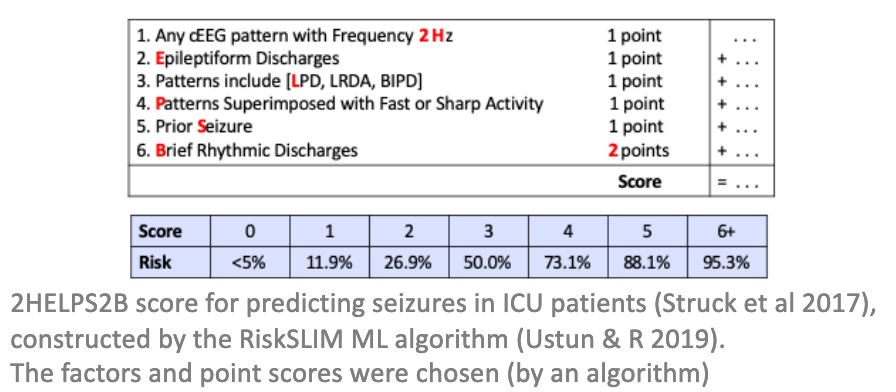
\includegraphics[width=\textwidth]{images/rudin_model.png}
\end{figure}
\end{frame}

\begin{frame}[c]{Interpretable Machine Learning (Cynthia Rudin)}
\begin{figure}
  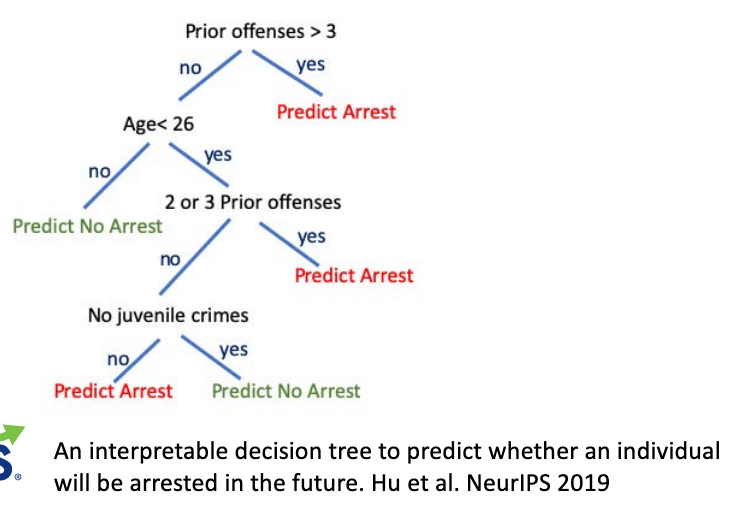
\includegraphics[width=\textwidth]{images/rudin_model_2.png}
\end{figure}
\end{frame}

\begin{frame}[c]{Interpretable Machine Learning}
Advantages:
\begin{itemize}
  \item Transparency makes it easy to detect reliance on context-specific proxies
  \item Also helpful for identifying bias
  \item Often perform as well as fancier methods
\end{itemize}
Disadvantages:
\begin{itemize}
  \item New? Have to go learn them? Honestly, I think we should all be using these.
\end{itemize}
\end{frame}

\begin{frame}[c]{Summary}
  \begin{itemize}
    \item Causal inference tends to be more robust
    \begin{itemize}
      \item Better when making \emph{bigger} extrapolations \\
      (e.g. if you plan to deliberately \alert{manipulate} the world!)
    \end{itemize}
    \item SML can be more powerful when you're sure your context won't change
    \begin{itemize}
      \item Training data looks just like data you want to work with
      \item World is unlikely to adapt to your model
    \end{itemize}
  \end{itemize}
\end{frame}

\end{document}
